\RequirePackage[l2tabu, orthodox]{nag}

%\documentclass[a4paper]{article}
%\documentclass[final, pdftex, a4paper, 12pt, openbib, ]{article}
\documentclass[final, pdftex, a4paper, openbib, ]{article}
\usepackage[utf8]{inputenc}
\usepackage[francais]{babel}
%\usepackage{lmodern}
\usepackage[T1]{fontenc}
%\usepackage{graphicx}
\usepackage{alltt}
\usepackage{float}
%\usepackage{times}
%\usepackage{a4wide}
\usepackage{upquote,textcomp}
\usepackage{geometry}
%\usepackage{hyperref}
\usepackage[
pdftex,
final,                      % if you do    want to have clickable-colorful links
pdfstartview = FitV,
linktocpage  = false,       % ToC, LoF, LoT place hyperlink on page number, rather than entry text
breaklinks   = true,        % so long urls are correctly broken across lines
% pagebackref  = false,     % add page number in bibliography and link to position in document where cited
]{hyperref}
\usepackage{mathtools}
\geometry{a4paper, portrait, margin=2cm}
%\addtolength{\textheight}{2 cm}
%\addtolength{\oddsidemargin}{-1cm}
%\addtolength{\topmargin}{-1cm}
%\addtolength{\textwidth}{1 cm}

%Good solution for monospaces
%\usepackage{pxfonts} % Or palatino or mathpazo, changes all fonts to something sans
%\usepackage{eulervm} % only changes math fonts, i checked
%\usepackage[ttdefault=true]{AnonymousPro} %Only changes tt fonts
% WHICH ONE TO CHOOSE?
\usepackage{pslatex}
%\usepackage[ttdefault=true]{AnonymousPro} %Only changes tt fonts
% \usepackage[varg, cmintegrals, cmbraces, ]{newtxtext,newtxmath} % libertine, uprightGreek (U.S.) or slantedGreek (ISO), 
% \usepackage{tgtermes}
% \usepackage{txfonts}
% \usepackage{mathptmx}
% \usepackage[scaled=.90]{helvet}
% \usepackage{courier}
% \usepackage{textcomp}     % required for special glyphs
% \usepackage{bm}   


\usepackage{caption}
\captionsetup[figure]{labelformat=empty}% redefines the caption setup of the figures environment in the beamer class.

%Inconsoloata, a little too light.
%\usepackage{inconsolata}
%\renewcommand{\ttdefault}{Consolas}
%\usepackage{fontspec} %Doesn't work with pdflatex
%\setmonofont{Consolas}



%\renewcommand*\familydefault{\ttdefault} %% Only if the base font of the document is to be typewriter style

%\newcommand\Fontvi{\fontsize{6}{7.2}\selectfont}

%Make tabularx center cells vertically
%\def\tabularxcolumn#1{m{#1}}
%\renewcommand{\tabularxcolumn}[1]{>{\small}m{#1}}

%%Syntax hilighting
%\usepackage{fancyvrb}
\usepackage{minted}
%\usepackage[newfloat]{minted}
\usemintedstyle{borland}
%\usepackage{etoolbox}
%\AtBeginEnvironment{minted}{\singlespacing%
%	\fontsize{14}{14}\selectfont}
%\newminted{java}{fontsize=\footnotesize}
\usepackage{caption}

%\usepackage{multicol}
%\usepackage{vwcol}
%\usepackage{lipsum}
%\usepackage{microtype}
%\setlength{\columnseprule}{0.4pt}
%\renewcommand{\columnseprulecolor}{\color{red}}
\newcommand{\BAD}[1]{{\color{red}#1}}
\newcommand{\GOOD}[1]{{\color{darkgreen}#1}}


\usepackage{graphicx}
\usepackage{colortbl,array}
\usepackage{tabularx}
\definecolor{warningbackground}{RGB}{252,226,158}

\newcommand{\alertwarningbox}[1]{
    \centering
    \begin{tabularx}{0.9\linewidth}{
        >{\columncolor{warningbackground}}c
        >{\columncolor{warningbackground}}X}
        \raisebox{\dimexpr2\baselineskip-\height}
        {
\includegraphics[scale=0.8]{attention.pdf}}&
        \raisebox{\tabcolsep}{\strut}#1\raisebox{-\tabcolsep}{\strut}
    \end{tabularx}
}


\usepackage{xcolor}

%\definecolor{infobackground}{RGB}{217,237,247}
%\definecolor{infoforeground}{RGB}{58,135,173}
%\definecolor{infoborder}{RGB}{188,232,241}

\definecolor{infobackground}{RGB}{217,237,247}
\definecolor{infoforeground}{RGB}{30,50,70}
\definecolor{infoborder}{RGB}{30,50,70}

\definecolor{infobackground}{RGB}{217,237,247}
\definecolor{infoforeground}{RGB}{30, 80, 150}
\definecolor{infoborder}{RGB}{47, 87, 232}


\usepackage{environ}
\usepackage{tikz}
\usetikzlibrary{fit,backgrounds,calc}

\NewEnviron{alertinfo}[1]
{
\begin{center}
    \begin{tikzpicture}
    \node[inner sep=0pt,
          draw=infoborder,
          line width=1pt,
          fill=infobackground] (box) {\parbox[t]{0.99\textwidth}
        {%
            \begin{minipage}{.12\textwidth}
                \centering\tikz[scale=3]
                \node[scale=1]
                {
%                    \includegrapTable de hachage, utilisation de bibliothèque
hics[scale=0.25]{\images/information.pdf}
                    
\includegraphics[scale=0.15]{\images/information.pdf}                    
                };
            \end{minipage}%
           \begin{minipage}{.86\textwidth}
%                \vskip 10pt
                \textbf{\textcolor{infoforeground}{\large #1}}\par\smallskip
                \textcolor{infoforeground}{\large \BODY}
                \par\smallskip
                \par\smallskip
            \end{minipage}\hfill
        }%
    };
    \end{tikzpicture}
\end{center}
}

\usepackage{titling}
\usepackage{soul}

\definecolor{Light}{gray}{.92}
\sethlcolor{Light}
\let\OldTexttt\texttt	
\renewcommand{\texttt}[1]{\OldTexttt{\hl{#1}}}

\newcommand{\codes}{../codes/TP9}
\newcommand{\images}{../images}

%\title{GBIAAL 4$^{\mbox{\`eme}}$ année \\ Devoir Surveillé --- Base de données \\ 13 janvier 2016  \\ 1 heure}
\title{IMA 3$^{\mbox{\`eme}}$ année\\ Programmation Avancé
	%\\TP1 Structures, Listes contiguës, Redirections}
}
\author{\huge \textbf{TP9 Table de hachage, utilisation de bibliothèque}}
\setlength{\parindent}{0pt}
\pagestyle{empty}
\date{}


\begin{document}
%\vspace{-15cm}
\posttitle{\par\end{center}}
\setlength{\droptitle}{-45pt}
\maketitle
%\thispagestyle{empty}

%\section{Schéma conceptuel}
\vspace{-1.7cm}
\section{Objectifs}

\begin{itemize}
	\item Savoir utiliser une bibliothèque
	\item Savoir construire une table de hachage et l'utiliser
\end{itemize}

%\paragraph{Contexte et préparation : } Avant de commencer, récupérez le fichier \url{~wrudamet/public/IMA3/TP6/tp6_gdb.tgz} à la ligne de commande. Désarchivez\footnote{Vous pouvez utiliser la commande \texttt{tar} pour décompresser et désarchivez ce fichier} le dans votre répertoire de \textit{Programmation Avancé} (toujours à la ligne de commande !).

\paragraph{Contexte et préparation : }
Dans ce TP, nous allons construire et utiliser une table de hachage. Les tables de hachage étant classiquement utilisées pour coder des dictionnaires, nous allons réaliser un dictionnaire anglais sommaire.

%\begin{alertinfo}{}
%	\textbf{IMPORTANT : Ce TP sera réutilisé dans le futur. Il servira d'inspiration pour le TP8 et votre librairie sera entièrement repris pour le TP9}
%\end{alertinfo}

\section{Questions du TP \large (à faire impérativement)}

\subsection{Récupération de fichiers}

\begin{enumerate}
	\item Récupérez votre librairie et votre fichier en-tête du TP7 (\texttt{listechaines.h} et \texttt{listechaines.a}).
	\item Copier les fichiers \texttt{hash.c}, \texttt{dico.english} et \texttt{Makefile} fournis dans \url{~wrudamet/public/IMA3/TP9/}
	\item Vérifier que le Makefile fonctionne : commande \texttt{make}.
	\item Lancer le programme (que fait-il?) et noter son temps d'exécution (commande \texttt{time}).
\end{enumerate}	


\subsection{Explications tables de hachage}
Lire attentivement l'annexe.


\subsection{Travail demandé}
	Dans le fichier fourni \texttt{hash.c} :

\begin{enumerate}
	\item Déclarer le type \texttt{Hashtable} (vecteur de taille \texttt{TABLE\_SIZE} de \texttt{Liste}).
	\item Écrire une fonction \texttt{void init\_ht(Hashtable ht)} qui initialise \texttt{ht} (listes à \texttt{NULL}).
	\item Écrire une fonction \texttt{void update\_ht(char *word, Hashtable ht)} qui ajoute \texttt{word} dans \texttt{ht} (fonction \texttt{ajout\_alphab} fournie) à la liste d'indice \texttt{hash(word)}.
	La fonction de hachage est fournie dans le \texttt{.c}.
	\item Écrire une fonction load\_ht(FILE *f, Hashtable ht) analogue à \texttt{charge\_fichier} qui charge les mots du fichier dans ht.
	\item Modifier la fonction \texttt{main} en remplaçant la liste par une Hashtable.
	\item Comparer les temps d'exécution avec la liste (version précédente)\footnote{N'oubliez pas de comparer ce qui est comparable en mettant en commentaire les traces ou affichages éventuels.}. Expérimenter avec des valeurs progressives de \texttt{TABLE\_SIZE} :\\
	\texttt{TABLE\_SIZE = 1} (vous devriez retrouver des performances très comparables)\\
	\texttt{TABLE\_SIZE = 10, 20, \ldots, 100, 200, 300, 400}
	\item Ecrire une fonction \texttt{void collisions(Hashtable ht)} qui affiche, pour chaque indice \texttt{i}, la taille de la liste \texttt{ht[i]}.
	Sur l'exemple, (avec \texttt{TABLE\_SIZE=50}) : %\\

%	\texttt{0 335}\\
%	\texttt{1 309}\\
%	\texttt{2 308}\\
%	\texttt{3 318}\\
%	\ldots
	\begin{minted}[mathescape=true,escapeinside=||,tabsize=4,
	%fontsize=\footnotesize,
	]{c}
	0 335
	1 309
	2 308
	3 318
	|\ldots|
	\end{minted}
	
\end{enumerate}

\section{Questions s'il vous reste du temps}
\begin{enumerate}
	\item Rediriger la sortie standard lors de l'exécution pour écrire le résultat de la fonction collision dans un fichier \texttt{trace.txt} (mettez en commentaire tout autre affichage).
	Visualiser la répartition des collisions avec \texttt{gnuplot} et faire de même avec différentes valeurs de \texttt{TABLE\_SIZE}.
\begin{minted}[mathescape=true,escapeinside=||,tabsize=4,
%fontsize=\footnotesize,
]{bash}
	./hash dico.english > trace.txt
	gnuplot
	gnuplot> plot "./trace.txt" with lines
\end{minted}
	Remarquer que la courbe ne change plus après \texttt{TABLE\_SIZE = 250} (environ).
	\item Déterminer la plus grande valeur de hachage possible du dictionnaire : Écrire une fonction : \texttt{void max\_hash(FILE *fp, char *max\_word, int *hmax)} qui détermine \texttt{hmax}, la plus grande somme de codes ascii des mots du dictionnaire, et fournit le mot correspondant dans \texttt{max\_word}.
	\item Afficher \texttt{max\_word} et \texttt{hmax}. Fixer \texttt{TABLE\_SIZE} à \texttt{hmax+1}, vous devez retrouver \texttt{max\_word} en affichant la liste de collisions d'indice \texttt{hmax}.
\end{enumerate}


\section{Annexes : Tables de hachage}

Une table de hachage est un compromis entre les listes chaînées efficaces sur les ajouts et les vecteurs (ou listes contiguës) efficaces sur les accès. Soit un ensemble fini $D$ de données (ici les mots du dictionnaire) que l'on va stocker dans un vecteur $ht$.
Pour ranger un élément $x$ de $D$, on calcule son image par une fonction de hachage $hash$, qui donne son indice (appelé \textit{indice de hachage}) dans $ht$, $x$ sera donc rangé dans $ht[hash(x)]$.
Il reste à trouver une fonction $hash$ adéquate :

\begin{itemize}
	\item L'idéal est de trouver une fonction \textbf{bijective} entre $D$ et l'intervalle d'indices du vecteur, ainsi chaque case du vecteur contient un élément de $D$. Mais il est difficile de trouver une telle fonction bijective, ne serait-ce que parce que $D$ est rarement connu a priori.

	\item L'utilisation d'une fonction \textbf{injective} (ie : qui associe à chaque $x$ de $D$ une case différente de $D$) mène à un vecteur de taille $sup\{hash(x)$, $x$ $\in$ $D$\}, c'est à dire un vecteur à trous, ce qui peut générer une perte importante de place.

	\item Le principe consiste alors à prendre une fonction \textbf{surjective} obtenue généralement par modulo sur une taille limitée de vecteur, soit $TABLE\_SIZE << card(D)$. On tombe alors sur un problème de \textit{« collisions »} parce que plusieurs données peuvent avoir le même indice de hachage.
	On choisit donc une structure mixte constituée d'un vecteur statique de listes chaînées contenant les éléments du même indice de hachage (appelées \textit{« listes de collisions »}).
	Si possible, ces listes sont ordonnées pour optimiser les accès.
	L'ajout d'un élément $x$ revient alors à calculer $hash(x)$ de coût quasi constant et insérer $x$ dans la liste $ht[hash(x)]$, en $O(n)$, $n$ étant la taille de la liste correspondante.
	Toute la difficulté est de trouver un bon compromis entre la taille du vecteur et taille des listes. Remarquez que prendre $TABLE\_SIZE=1$ revient à faire une simple liste.
\end{itemize}

\begin{minipage}{1\textwidth}
		\vspace{1cm}
       	\centering\tikz[scale=3]
       	\node[scale=1]
       	{
       		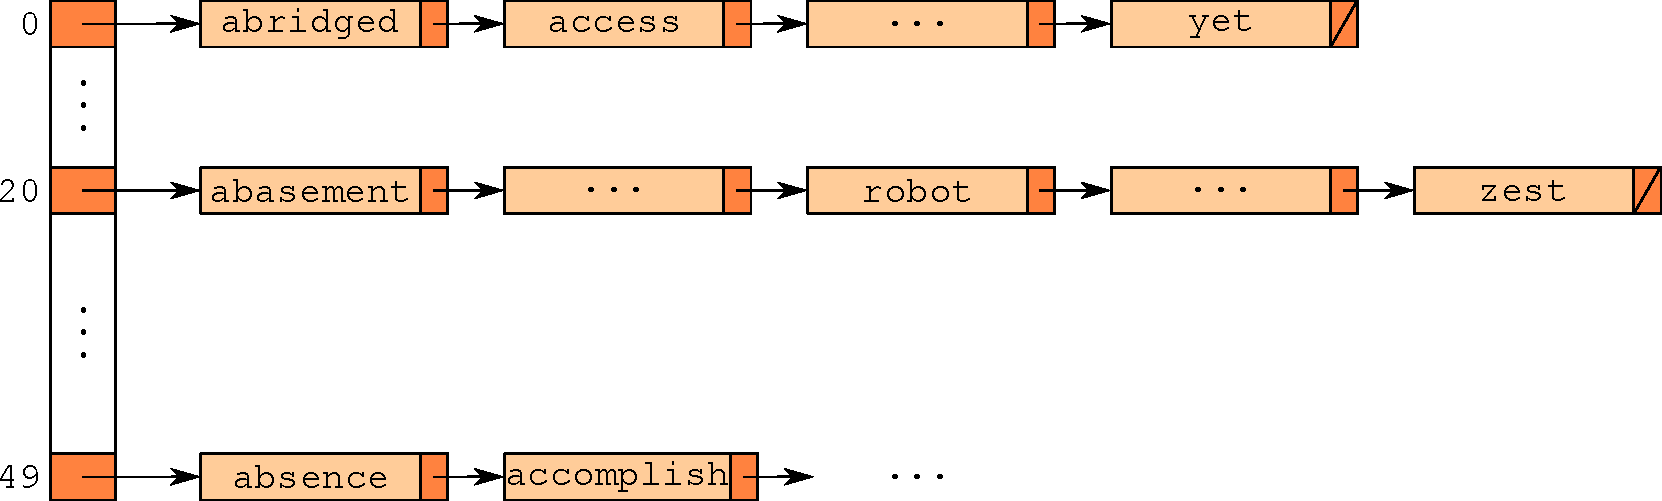
\includegraphics[scale=0.58]{hashtable.pdf}
       		%                    
\includegraphics[scale=0.15]{\images/information.pdf}                    
       	};
\end{minipage}%


\end{document}
